%!TeX root=../tese.tex
\chapter{Álgebras de flag}
\label{cap:flag-algebras}

\newcommand{\emptyflag}{\varnothing}
\newcommand{\isom}{\cong}

% Tikz setup from https://arxiv.org/abs/2103.14179

\newcommand{\vc}[1]{\ensuremath{\vcenter{\hbox{#1}}}}
\tikzset{vtx/.style={inner sep=1.7pt, outer sep=0pt, circle, fill}}
\tikzset{unlabeled_vertex/.style={inner sep=1.7pt, outer sep=0pt, circle, fill, draw=black}}
\tikzset{labeled_vertex/.style={inner sep=2.2pt, outer sep=0pt, rectangle, fill=yellow, draw=black}}
\tikzset{edge_color0/.style={color=black,line width=1.2pt}}
\tikzset{edge_color1/.style={color=red,  line width=1.2pt,opacity=0}}
\tikzset{edge_color2/.style={color=blue, line width=1.2pt,opacity=1}}

\newcommand{\flagone}{ % this is the unlabeled triangel
  \vc{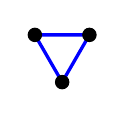
\begin{tikzpicture}[scale=0.5]
    \draw \foreach \x in {0,1,2}{(270+\x*360/3:0.8) coordinate(x\x)};
    \draw[edge_color2] (x0)--(x1)--(x2)--(x0);
    \draw (x0) node[unlabeled_vertex]{};
    \draw (x1) node[unlabeled_vertex]{};
    \draw (x2) node[unlabeled_vertex]{};
  \end{tikzpicture}}
}
\newcommand{\kthree}{\flagone}

\newcommand{\flagtwo}{ % this is the unlabeled edge
  \vc{
\begin{tikzpicture}[scale=0.5]
    \draw (225:0.8) coordinate(x0);
    \draw (45:0.8) coordinate(x1);
    \draw[edge_color2] (x0)--(x1);
    \draw (x0) node[unlabeled_vertex]{};
    \draw (x1) node[unlabeled_vertex]{};
  \end{tikzpicture}}
}
\newcommand{\edge}{\flagtwo}

\newcommand{\flagthree}{
  \vc{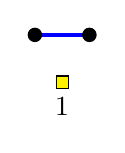
\begin{tikzpicture}[scale=0.5]
    \draw \foreach \x in {0,1,2}{(270+\x*360/3:0.8) coordinate(x\x)};
    \draw[edge_color2] (x1)--(x2);
    \draw (x0) node[labeled_vertex,label=below:$1$]{};
    \draw (x1) node[unlabeled_vertex]{};
    \draw (x2) node[unlabeled_vertex]{};
  \end{tikzpicture}}
}

\section{Preliminares}

Seja $k \geq 0$ um inteiro.
Um \emph{tipo} de \emph{tamanho} $k$ é um grafo $G$ com $V(G) = [k]$,
i.e. é um grafo com todos os seus vértices rotulados.
O tipo vazio é denotado por $\emptyflag$.

Seja $\sigma$ um tipo de tamanho $k$.
Um \emph{$\sigma$-flag} é um par $(F,\phi)$ em que $\phi \colon [k] \to V(F)$
é um homomorfismo de grafos injetor tal que $F[\phi([k])] \isom \sigma$.


\begin{example}[Mantel]
  Se $\kthree = 0$, então $\edge \leq \frac12$.
\end{example}


\section{Aplicações para a Conjectura \ref{conj:make-bipartite}}

\begin{theorem}
  Se $\kthree = 0$ e $\edge \geq \frac{2}{25}$, então
  $\left\llbracket
  \flagthree
  \right\rrbracket
  \leq \frac{2}{25}$.
\end{theorem}

\begin{corollary}
  Seja $G$ um grafo com $n$ vértices e pelo menos $\frac{n^2}{5}$ arestas.
  Então a Conjectura \ref{conj:make-bipartite} vale para $G$.
\end{corollary}

O ponto é que ter a linguagem de flag algebras facilita obter cotas a partir da ideia de ``cortes locais'' e daí pode automatizar o processo.

\begin{theorem}[Balogh-Clemen-Lidický]
  Seja $G$ um grafo livre de triângulos com $n$ vértices.
  Então, vale que
  \begin{enumerate}
    \item $D(G) \leq \frac{n^2}{23.5}$;
    \item $D(G) \leq \frac{n^2}{25}$ se $e(G) \geq 0.3197 \binom{n}{2}$;
    \item $D(G) \leq \frac{n^2}{25}$ se $e(G) \leq 0.2486 \binom{n}{2}$.
  \end{enumerate}
\end{theorem}